%!TEX root = ../memoria.tex

\chapter{Gestión de calidad}

\section{Equipo de trabajo}

A continuación, se presenta un esquema que muestra la estructura del equipo de trabajo basado en \citet{web00}\\ 

\begin{figure}[ht!]
\centering
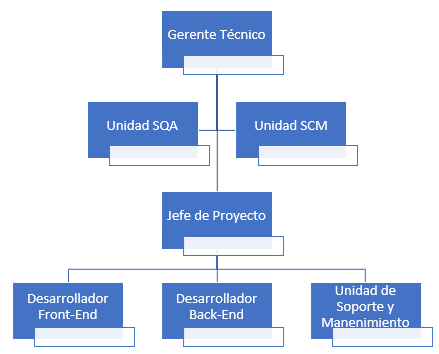
\includegraphics[width=.7\textwidth]{figures/equipo-trabajo.png}
\caption{Equipo de trabajo}
\label{fig:Equipo de trabajo}
\end{figure}

Según Don Wells, autor de las reglas de \textit{Extreme Programming},  el equipo debe tener dos características transversales:

	\begin{itemize}
		\item 
		 \textbf{Coraje}: Se debe ser sincero respecto al progreso y plazos del proyecto. Los trabajadores forman parte de un equipo, por lo que no deben temer a nada.
		\item
		 \textbf{Respeto}: Se debe respetar a todos los miembros del equipo y clientes. Cada trabajador realiza un aporte valioso al equipo, por lo que debe ser respetado.
	\end{itemize}

\section{Recursos}
\subsection{Personal}
\subsubsection{Gerente Técnico}

Las responsabilidades del gerente técnico son:

	\begin{itemize}
		\item 
		 Establecer y seleccionar el lineamiento de un programa de calidad para el desarrollo de \textit{software}.
		\item
		 Revisar y aprobar el plan de \textit{SQA} para cada proyecto. 
		 \item
		 Facilitar al equipo los medios para la realización de las actividades asociadas al plan de \textit{SQA}.
		 \item 
		 Monitorear las actividades de \textit{SQA}.
	\end{itemize}

\subsubsection{Unidad \textit{SQA}}

Son los encargados de generar el plan de aseguramiento de calidad que incluyen el aseguramiento de calidad de entregables y la documentación. Si bien, son los encargados de realizar el plan de calidad, no son encargados de velar por la realización de las actividades asociadas al plan o de prácticas, procesos y procedimientos. Dicha responsabilidad recae en el jefe de proyecto y encargados de cada área.

Las responsabilidades de la unidad de \textit{SQA} son: 

	\begin{itemize}
		\item 
		 Establecer los estándares de calidad.
		\item
		 Observar, participar y verificar que las revisiones de calidad se realicen correctamente. 
		 \item
		Velar por la correcta realización de las distintas pruebas y procedimientos establecidos de acuerdo con el plan de pruebas.
		 \item 
		Crear un plan de identificación de defectos para el proceso de desarrollo y apoyar a áreas de gestión en perfeccionar estos.
	\end{itemize}

\subsubsection{Unidad \textit{SCM}}

La unidad de Gestión de Configuración del \textit{Software} es la encargada de mantener la integridad del producto a lo largo de todo el desarrollo del proyecto, mediante un control de cambios adecuado para el desarrollo.

Las responsabilidades de \textit{SCM} asociadas a \textit{SQA} son: 

	\begin{itemize}
		\item 
		Revisar y comentar el plan de \textit{SQA} para el proyecto. 
		\item
		Implementar las actividades de calidad de acuerdo con el plan de \textit{SQA}. 
		 \item
		Resolver los problemas detectados por \textit{SQA} relacionados con \textit{SCM}.
		 \item 
		Implementar las prácticas, procesos y procedimientos definidos en el plan de \textit{SCM} y en otros planes o documentos complementarios.
	\end{itemize}

\subsubsection{Jefe de Proyecto}

Las responsabilidades del jefe de proyecto son:

\begin{itemize}
		\item 
		Establecer un programa de calidad para el proyecto de desarrollo de \textit{software} de acuerdo con las políticas organizacionales.
		\item
		Identificar las actividades de \textit{SQA} requeridas para el proyecto.
		\item
		Revisar y aprobar el plan de \textit{SQA} para el proyecto.
		\item 
		Identificar los participantes de las actividades de \textit{SQA}.
		\item
		Implementar las actividades de \textit{SQA} de acuerdo con el plan.
		\item
		Monitorear las actividades de \textit{SQA} planificadas en el plan.
		\item
		Identificar los factores de calidad para la implementación del software.
		\item
		Identificar, desarrollar y mantener la documentación del proyecto. 
	\end{itemize}

\subsubsection{Desarrolladores \textit{Front-End}, Desarrolladores \textit{Back-End} y Soporte y mantenimiento}

El área de soporte y mantenimiento es el encargado de realizar correcciones y solucionar problemas relacionados con el adecuado funcionamiento del sistema una vez este se encuentre en ambientes productivos. Esto se traduce en identificar causas de errores mediante el registro de actividades de la aplicación y dar soporte a consultas del cliente.

Por otro lado, el área de desarrollo se divide en desarrolladores \textit{Front-End} y \textit{Back-End} que hace referencia a la capa del sistema sobre la cual realizan su trabajo de desarrollo. 

El desarrollador \textit{Front-End} trabaja sobre la capa de presentación de datos, es decir, la que interactúa directamente con el usuario. Mientras el desarrollador \textit{Back-End} trabaja sobre la capa de acceso de datos que se encarga de procesar la información proveniente de la capa de presentación

Sus responsabilidades con \textit{SQA} son: 

	\begin{itemize}
		\item
		Revisar y entregar sus observaciones sobre el plan de \textit{SQA} para el proyecto.
		\item
		Implementar las actividades de \textit{SQA} de acuerdo con el plan.
		\item
		Participar de la solución de los problemas detectados por las actividades de \textit{SQA} que sean de su competencia.
		\item
		Implementar las prácticas, procesos y procedimientos definidos en el plan de proyecto y en otros planes o documentos complementarios.
	\end{itemize}

\subsection{Infraestructura}
Para un buen desarrollo del sistema, además de los recursos humanos y la realización de las actividades de \textit{SQA} es necesario contar una infraestructura que pueda satisfacer las necesidades del equipo para la realización del software. 

\subsubsection{Oficina}

Es necesaria una oficina que posea áreas de trabajo y salas de reuniones. Respecto a las áreas de trabajo estas deben contar con escritorios y sillas ergonómicas recomendadas para trabajo de escritorio que cuenten con altura variable y soporte para brazos y espalda. Los escritorios deben tener un largo no inferior a un metro y un ancho no inferior a 70 cm. 

Respecto a las oficinas de reuniones, esta debe tenera disposición un televisor que permita conexión a un equipo (\textit{notebook} o dispositivo móvil) o en su defecto un proyector.

Es necesario que en la oficina existan los servicios básicos como luz y agua potable. Finalmente es necesario contar con una conexión de internet no menor de 50 Mbps.

\subsubsection{Equipamiento de trabajo}

Es necesario mínimo de 5 equipos de trabajo enfocados en el desarrollo.

	\begin{itemize}
		\item 
		\textbf{Procesador}: Intel Core i7-7700.
		\item 
		\textbf{Memoria}: 12GB DDR4 (2400 MHz).
		\item 
		\textbf{Almacenamiento}: Unidad SSD 240GB Lectura 540 MB/s Escritura 465 MB/s.
		\item 
		\textbf{Pantalla}: Dos pantallas de mínimo 17”.
	\end{itemize}

Además, es necesario  3 equipos Laptop para uso administrativo. 

	\begin{itemize}
		\item 
		\textbf{Procesador}: Intel Core i5 7200U.
		\item 
		\textbf{Memoria}: 8GB DDR4 (2400 MHz).
		\item 
		\textbf{Almacenamiento}: HDD 1TB (5400rpm).
	\end{itemize}

\subsection{Actividades}

El área de \textit{SQA}, con el objetivo de asegurar la calidad de forma continua, se debe encargar de varias actividades a lo largo del proceso de desarrollo de \textit{Gerprin}. Es importante que \textit{SQA} realice las definiciones de estándares, revisión de productos y procesos, pruebas y análisis de defectos hasta la entrega exitosa de las últimas modificaciones y posteriores documentaciones del sistema. Para esto, debe trabajar en conjunto con las áreas de desarrollo, tanto \textit{Front-End}, \textit{Back-End}, unidades de soporte, mantenimiento e implantación.

Las siguientes actividades se encuentran basadas en Herramientas específicas para el grupo de \textit{SQA} \citet{web00}.

\subsubsection{Evaluación de la selección de los productos de trabajo}

El \textit{SQA} debe asistir al jefe de proyectos en la elaboración de los estándares y guías aplicables que conforman los distintos artefactos necesarios para la planificación inicial del proyecto. Entre los elementos que deben ser considerados son herramientas por utilizar, diseño preliminar y \textit{mockup} de la interfaz del sistema, entre otros.

\subsubsection{Evaluación de las herramientas} 

En esta actividad el \textit{SQA} tiene la responsabilidad de evaluar las herramientas que serán empleadas para el desarrollo del sistema, considerando herramientas para pruebas, evaluaciones de rendimiento de la aplicación y herramientas de administración de proyectos.

Por otro lado, junto con el jefe de proyecto deben ser decididas las herramientas empleadas directamente en el proceso de desarrollo como \textit{frameworks}, herramientas de despliegue de aplicaciones, entre otros.

\subsubsection{Evaluación de la planificación y el monitoreo del proyecto}

\textit{SQA} es responsable de la elaboración del plan de aseguramiento de calidad, la elaboración e identificación de guías y estándares que puedan ser aplicados a las iteraciones y entregables.

\subsubsection{Evaluación de la especificación de requerimientos}

Respecto a las especificaciones de requerimiento \textit{SQA} debe realizar las siguientes actividades:

	\begin{itemize}
		\item 
		Verificar que se cumplan correctamente las actividades y procesos de la fase de exploración.
		\item
		Garantizar que se revisaron adecuadamente los entregables (especificación del sistema y de requerimientos) de la fase de exploración. 
		\item
		Asegurar la inclusión de la corrección de los entregables según las observaciones realizadas en el proceso de revisión. 
		\item
		Corroborar que estén expresados y documentados los requerimientos funcionales, técnicos, operacionales y de interfaz, de manera tal que puedan ser verificados en el producto final.
	\end{itemize}

\subsubsection{Evaluación del diseño}

\textit{SQA} es responsable de:

	\begin{itemize}
		\item 
		Garantizar que se revisaron adecuadamente los entregables (diseño preliminar, plan de pruebas, especificación de casos y procedimientos de prueba) de la fase de planificación de las entregas e iteraciones.
		\item
		Asegurar la inclusión de la corrección de los entregables según las observaciones realizadas en el proceso de revisión.
	\end{itemize}
	
\subsubsection{Evaluación de la implementación y de la prueba de unidad}

\textit{SQA} debe:

	\begin{itemize}
		\item 
		Garantizar que el proceso de codificación, las revisiones asociadas y la prueba de unidad sean conducidos de acuerdo a lo señalado en el plan de pruebas.
		\item
		Asegurar la inclusión de la corrección de los entregables según las observaciones realizadas en el proceso de revisión.
		\item
		Verificar la implementación de las acciones correctivas derivadas de la prueba de unidad.
		\item
		Comprobar la utilización de la especificación de procedimientos y casos de prueba durante la prueba de unidad. 
		\item
		Corroborar la documentación del código y de los resultados de la prueba de unidad.
	\end{itemize}

\subsubsection{Evaluación de la integración y prueba}

\textit{SQA} es responsable de:

	\begin{itemize}
		\item 
		Verificar que el proceso de integración y las actividades de prueba sean realizadas conforme al plan de proyecto, el diseño, el plan de prueba y los estándares y procedimientos establecidos.
		\item
		Asegurar que la prueba de integración haya sido completada satisfactoriamente, que sus resultados fueron registrados y divulgados y que las acciones correctivas derivadas de ella fueron implementadas.
		\item	
		Corroborara el desarrollo adecuado de las pruebas de aceptación y del sistema.
		\item
		Monitorear las actividades de prueba y certificar sus resultados.
		\item
		Revisar las pruebas.
	\end{itemize}

\subsubsection{Evaluación del producto antes de su liberación}

Se deben realizar las evaluaciones del producto terminado y la documentación. Para esto es necesario que el área de \textit{SQA} sea participe de las auditorias.

\subsubsection{Evaluación del proceso de revisión}

\textit{SQA} es responsable de garantizar que todos los entregables sean revisados y corregidos en caso de ser necesario y analizar los problemas encontrados de una forma sistémica, identificando causas, impactos y frecuencia de ocurrencia.

\subsubsection{Evaluación de las acciones correctivas}

\textit{SQA} es responsable de establecer acciones preventivas y monitorear que estas sean implementadas de forma correcta. 

\subsubsection{Evaluación del proceso de \textit{SCM}}

\textit{SQA} debe:

\begin{itemize}
		\item 
		Revisar el plan de \textit{SCM}.
		\item 
		Asegurar la correcta identificación de los ítems de configuración.
		\item 
		Garantizar un adecuado control de cambios.
		\item 
		Corroborar que la contabilidad del estado de la configuración sea preparada oportunamente y que refleje la situación real de los ítems de configuración en relación con el proyecto.
		\item 
		Comprobar la adherencia de las actividades de \textit{SCM} al plan de \textit{SCM}.
		\item 
		Verificar el correcto funcionamiento de la librería del \textit{software}.
	\end{itemize}

\subsubsection{Verificar la implementación de los procesos}

\textit{SQA} debe velar por la correcta implementación y cumplimiento de estándares y procesos definidos en las especificaciones de requisitos y planificación de iteraciones.

\subsubsection{Establecer las auditorías}

\textit{SQA} es responsable en la institución por el desarrollo de las auditorías internas. Por lo tanto, debe gestionarlas de ser preciso.

\subsubsection{Responsabilidades}

El área de \textit{SQA} es responsable de revisar que los productos de trabajo se adecuen a los estándares, procedimientos y al plan de proyecto, además de dar seguimiento a las actividades realizadas a lo largo del desarrollo del proyecto. Todo lo anteriormente observado debe ser informado al jefe de proyecto y de ser necesario al jefe de proyecto.

En la siguiente tabla se adjunta la matriz de responsabilidades \citet{web00}.

\begin{table}[H]
    \caption[Responsabilidades por actividades.] {Responsabilidades por actividades.}
    \label{tbl:responsabilidades por actividades}
    \begin{tabular}{|p{.58\textwidth}|p{.02\textwidth}|p{.02\textwidth}|p{.02\textwidth}|p{.02\textwidth}|p{.02\textwidth}|p{.02\textwidth}|p{.02\textwidth}|p{.02\textwidth}|}
        \hline
        \textbf{Actividad} &  \begin{sideways}\textbf{GT}\end{sideways} & \begin{sideways}\textbf{JP}\end{sideways} & \begin{sideways}\textbf{SQA}\end{sideways} & \begin{sideways}\textbf{SCM}\end{sideways} & \begin{sideways}\textbf{Analista}\end{sideways} & \begin{sideways}\textbf{Front-End}\end{sideways} & \begin{sideways}\textbf{Back-End}\end{sideways} & \begin{sideways}\textbf{Tester}\end{sideways}\\
    	\hline
    	\hline
    	Evaluación	de la selección los productos de trabajo. & X & X & X & X & X & & & \\ \hline
    	Evaluación de las herramientas & X & X & X & & & & & \\ \hline
    	Evaluación de la planificación y el monitoreo del proyecto & X & X & X & X & & & & \\ \hline
    	Evaluación de la especificación de requerimientos & X & X & X & & X & X & X & X \\ \hline
    	Evaluación del diseño & X & X & X & & X & X & X & X \\ \hline
    	Evaluación de la implementación y de la prueba de unidad & & & X & & & X & X & X \\ \hline
    	Evaluación de la integración y prueba & & & X & & & X & X & X \\ \hline
    	Evaluación del producto antes de su liberación & & X & X & & X & X & X & X \\ \hline
    	Evaluación del proceso de revisión & & X & X & & & & & \\ \hline
    	Evaluación de las acciones correctivas & X & X & X & X & & & & \\ \hline
    	Evaluación del proceso de \textit{SCM} & X & X & X & X & & & & \\ \hline
    	Verificar la implementación de los procesos & & X & X & & & & & \\ \hline
    	Establecer las auditorías & & X & X & X & & & & \\ \hline
    	
    \end{tabular}
\end{table}















	



